\documentclass[12pt,a4paper]{article}

\usepackage[T1]{fontenc}
\usepackage[utf8]{inputenc}
\usepackage[top=2.5cm,bottom=2.5cm,left=2.5cm,right=2.5cm]{geometry}
\usepackage[most]{tcolorbox}
\tcbuselibrary{breakable}
\usepackage{pgfplots}
\pgfplotsset{compat=1.18}
\usepackage{tikz}
\usetikzlibrary{arrows.meta,positioning}
\usepackage{booktabs}
\usepackage{parskip}
\usepackage{lmodern}
\usepackage{microtype}
\usepackage{xcolor}
\usepackage{enumitem}
\usepackage[colorlinks=true,linkcolor=blue,urlcolor=blue]{hyperref}

% ------------------------------------------------------------------
% Colour palette
% ------------------------------------------------------------------
\definecolor{csblue}{HTML}{1E5FA8}
\definecolor{csbluebg}{HTML}{EEF4FF}
\definecolor{amber}{HTML}{C8900A}
\definecolor{amberbg}{HTML}{FFFBEA}
\definecolor{green}{HTML}{2E8B57}
\definecolor{greenbg}{HTML}{F0FFF0}
\definecolor{rose}{HTML}{C2185B}
\definecolor{rosebg}{HTML}{FFF0F5}

% ------------------------------------------------------------------
% Box definitions
% ------------------------------------------------------------------
\newtcolorbox{casestudybox}[1]{
  colback=csbluebg, colframe=csblue,
  colbacktitle=csblue, coltitle=white,
  title={\textbf{Case Study:} #1},
  fonttitle=\small\bfseries,
  breakable, enhanced,
  boxrule=0.8pt, arc=4pt,
  left=8pt, right=8pt, top=6pt, bottom=6pt
}

\newtcolorbox{didyouknow}[1]{
  colback=amberbg, colframe=amber,
  colbacktitle=amber, coltitle=white,
  title={\textbf{Did You Know?} \textnormal{#1}},
  fonttitle=\small\bfseries,
  breakable, enhanced,
  boxrule=0.8pt, arc=4pt,
  left=8pt, right=8pt, top=6pt, bottom=6pt
}

\newtcolorbox{workedexample}[1]{
  colback=greenbg, colframe=green,
  colbacktitle=green, coltitle=white,
  title={\textbf{Worked Example:} #1},
  fonttitle=\small\bfseries,
  breakable, enhanced,
  boxrule=0.8pt, arc=4pt,
  left=8pt, right=8pt, top=6pt, bottom=6pt
}

\newtcolorbox{thinkabout}{
  colback=rosebg, colframe=rose,
  colbacktitle=rose, coltitle=white,
  title={\textbf{Think About It}},
  fonttitle=\small\bfseries,
  breakable, enhanced,
  boxrule=0.8pt, arc=4pt,
  left=8pt, right=8pt, top=6pt, bottom=6pt
}

\setlength{\parindent}{0pt}
\setlength{\parskip}{8pt}

% ==================================================================
\begin{document}
% ==================================================================

\section*{Exchange Rate Systems}

We learnt about the exchange rates, how they influence our life, and what makes the Indian Rupee appreciate or depreciate. But how are exchange rates actually determined, and what exchange systems have been used in history? To answer this we first need to understand the different types of exchange rate systems.

\subsection*{Types of Exchange Rate Systems}

An exchange rate system is how a country governs the valuation of its currency relative to others. There are three main types:

\begin{enumerate}[leftmargin=*, label=\arabic*.]

\item \textbf{Fixed Exchange Rate System:} In a fixed (or pegged) system, a country's monetary authority sets and upholds a constant value of its currency against another currency, a basket of currencies, or a commodity like gold. Central banks intervene by buying or selling foreign currency to keep the rate steady. The main advantage is certainty and stability, which helps businesses that trade across borders and keeps inflation in check. However, it requires the country to hold large reserves of foreign currency to defend the fixed rate, and if the rate is set incorrectly, it can lead to economic crises like the one India faced in 1991.

\item \textbf{Floating Exchange Rate System:} In a floating system, the currency's value is determined purely by market supply and demand, with little to no direct government control. These systems are self-correcting, as exchange rate adjustments reduce trade imbalances over time. The advantage is that the government does not need large reserves and the currency reflects the true state of the economy. The disadvantage is that rates can be volatile and unpredictable, making it harder for businesses to plan.

\item \textbf{Managed Floating (Dirty Float) Exchange Rate System:} This is a hybrid of the two systems above. Currency values are primarily set by the market, but the central bank occasionally steps in to prevent extreme swings. The benefit is flexibility combined with a safety net. The drawback is that interventions can be unpredictable, and there is a risk of governments using them to artificially weaken their currency for trade advantages.

\end{enumerate}

\begin{thinkabout}
Do you know which of these three systems India uses today? As you read through the history below, see if you can identify the moment India switched to its current system.
\end{thinkabout}

% ------------------------------------------------------------------
% CASE STUDY: History 1947-1992
% ------------------------------------------------------------------

\begin{casestudybox}{India's Exchange Rate Regimes, 1947--1992}

India's approach to managing the Rupee went through five distinct phases before it arrived at the managed float used today. Each change was driven by a combination of global events and domestic pressures.

\medskip

% Timeline
\begin{center}
\resizebox{0.97\linewidth}{!}{%
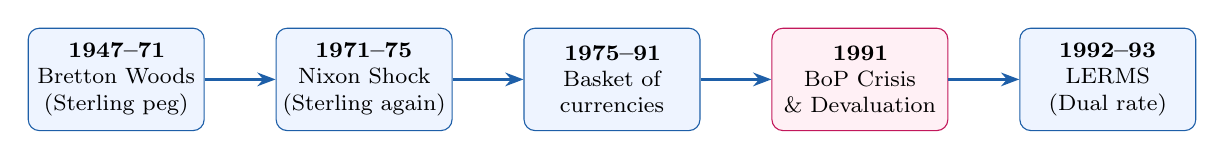
\begin{tikzpicture}[
  era/.style={
    draw=csblue, fill=csbluebg,
    rounded corners=4pt,
    text width=2.0cm, align=center,
    minimum height=1.3cm,
    font=\footnotesize
  },
  arr/.style={-Stealth, thick, color=csblue}
]
  \node[era] (a) {\textbf{1947--71}\\Bretton Woods\\(Sterling peg)};
  \node[era, right=0.9cm of a] (b) {\textbf{1971--75}\\Nixon Shock\\(Sterling again)};
  \node[era, right=0.9cm of b] (c) {\textbf{1975--91}\\Basket of\\currencies};
  \node[era, draw=rose, fill=rosebg, right=0.9cm of c] (d) {\textbf{1991}\\BoP Crisis\\\& Devaluation};
  \node[era, right=0.9cm of d] (e) {\textbf{1992--93}\\LERMS\\(Dual rate)};

  \draw[arr] (a.east) -- (b.west);
  \draw[arr] (b.east) -- (c.west);
  \draw[arr] (c.east) -- (d.west);
  \draw[arr] (d.east) -- (e.west);
\end{tikzpicture}}
\end{center}

\medskip

\textbf{1947--1971: Bretton Woods and the Sterling Peg}

After Independence in 1947, India joined the Bretton Woods system, under which the U.S. Dollar was pegged to gold at \$35 per ounce and all other currencies were pegged to the Dollar. India chose to use the British Pound Sterling as its intervention currency rather than the Dollar, largely because of its longstanding economic and colonial ties with Britain. The Rupee was fixed at approximately Rs.\,4.76 per Dollar.

\medskip
\textbf{1971--1975: The Nixon Shock}

In 1971, the U.S. government ended its commitment to convert Dollars into gold, an event known as the Nixon Shock, which caused the Bretton Woods system to collapse. India briefly shifted its peg to the U.S. Dollar in August 1971, but reverted to the British Pound Sterling in December of the same year. This was beneficial because the Sterling's depreciation allowed the Rupee to depreciate with it, improving India's export competitiveness during the global oil crisis.

\medskip
\textbf{1975--1991: A Basket of Currencies}

When the Sterling itself became unstable in the mid-1970s, India moved away from pegging to a single currency. In 1975, the RBI linked the Rupee to a weighted basket of its major trading partners' currencies, including the U.S. Dollar, British Pound, Deutsche Mark, Japanese Yen, and French Franc. This made the Rupee more stable, since weakness in one currency could be offset by strength in others. However, by the late 1980s, India was spending far more on imports than it earned from exports and borrowing heavily to cover the gap, setting the stage for crisis.

\medskip
\textbf{1991: The Balance of Payments Crisis}

By 1991, India's foreign exchange reserves had fallen so low that the country could barely pay for two weeks of imports. The government was forced to pledge 67 tonnes of gold to the Bank of England and the Bank of Japan to secure emergency funds. To restore export competitiveness, the Rupee was devalued by approximately 18--20\% against the Dollar over just three days (July 1--3, 1991), and a broader programme of economic liberalisation was launched.

\medskip
\textbf{1992--1993: The Dual Rate System (LERMS)}

As a bridge to a fully market-determined system, India introduced the Liberalised Exchange Rate Management System (LERMS) in March 1992. Exporters were required to surrender 40\% of their foreign exchange earnings to the RBI at a fixed official rate, while the remaining 60\% could be converted at the market rate. This transitional arrangement lasted only until March 1993, when the two rates were unified into a single market-determined rate.

\end{casestudybox}

\subsection*{India's Current Exchange Rate System: 1993 to the Present}

Since March 1993, India has operated under a market-determined exchange rate, known as a managed float. The dual exchange rate system was abolished, and the value of the Rupee became primarily set by the forces of supply and demand. This makes it a managed floating system, the same hybrid model described in point 3 above.

Under this system, the RBI does not fix the Rupee's value, but it does intervene from time to time by buying or selling foreign exchange to prevent excessive or abrupt fluctuations. In 1994, India also made the Rupee fully convertible on the current account, meaning individuals and businesses could freely exchange Rupees for foreign currencies for trade in goods, services, and income, without needing prior government approval. However, full convertibility on the capital account (for investments and borrowings) is still not in place, and the RBI carefully regulates those flows to maintain financial stability.

% ==================================================================
\section*{The RBI and India's Foreign Exchange Reserves}
% ==================================================================

We have seen how the RBI intervenes in the foreign exchange market to stabilise the Rupee. But what exactly does it intervene with? The answer lies in India's \textbf{foreign exchange reserves}, a stockpile of assets that the RBI holds and manages on behalf of the country.

India's foreign exchange reserves are made up of four components. The largest part is \textbf{foreign currency assets}, holdings of major currencies like the U.S. Dollar, Euro, and Pound Sterling, typically invested in safe foreign government securities. The second component is \textbf{gold}. The third is \textbf{Special Drawing Rights (SDR)}, an international reserve asset created by the IMF that member countries can use to settle payments with other nations. The fourth is \textbf{India's reserve position with the IMF}, the amount India can draw on demand without conditions.

Why does a country hold these reserves? There are three main reasons. First, they act as a buffer against economic shocks: if exports collapse or a financial panic hits, reserves can cushion the blow. Second, they ensure the country can pay for its imports even during difficult times. A commonly used measure is \textbf{import cover}, which tells us how many months of imports a country could pay for using only its reserves. Third, large reserves signal financial stability to foreign investors, encouraging investment.

\begin{didyouknow}{From Crisis to Confidence}
In mid-1991, India's usable foreign exchange reserves fell to roughly \$1.2 billion, enough to cover less than three weeks of imports. By 2024, India's reserves stood at over \$640 billion, covering approximately 10--11 months of imports. That is a turnaround of over 500 times in just 33 years.

\smallskip
{\footnotesize \textit{Sources: Wikipedia (1991 Indian economic crisis); Deccan Chronicle; World Bank Total Reserves series.}}
\end{didyouknow}

The chart below shows how India's foreign exchange reserves have grown since 1991.

\begin{center}
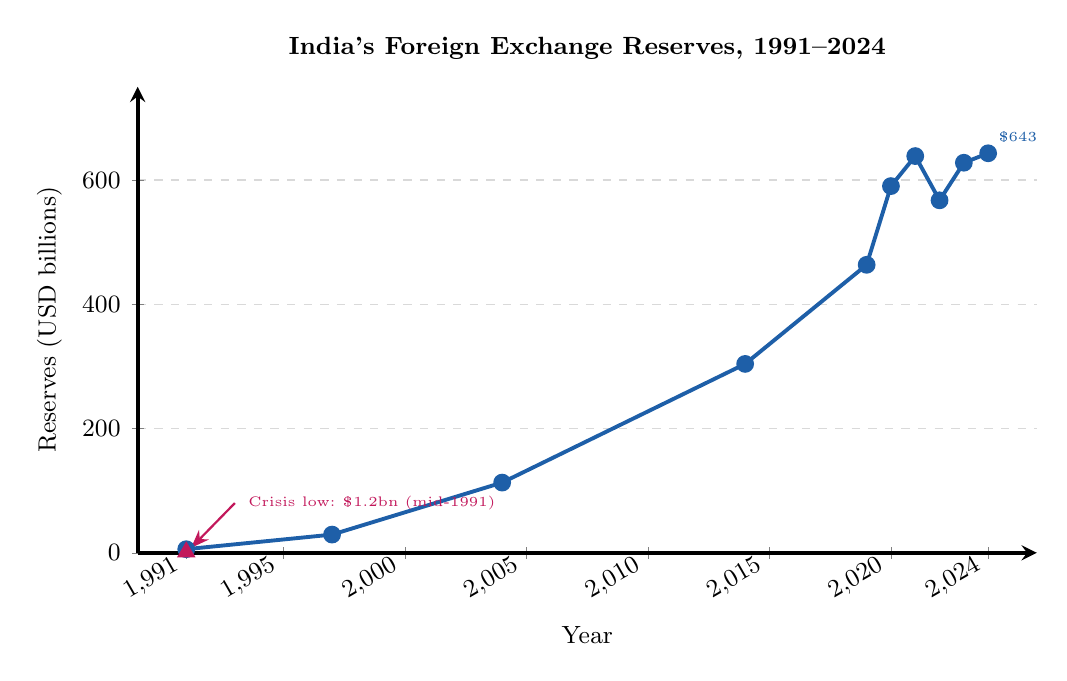
\begin{tikzpicture}
\begin{axis}[
  width=13cm, height=7.5cm,
  xlabel={Year},
  ylabel={Reserves (USD billions)},
  xmin=1989, xmax=2026,
  ymin=0, ymax=750,
  xtick={1991,1995,2000,2005,2010,2015,2020,2024},
  xticklabel style={font=\small, rotate=30, anchor=east},
  yticklabel style={font=\small},
  ymajorgrids=true,
  grid style={dashed, gray!30},
  axis lines=left,
  line width=1.4pt,
  mark size=2.5pt,
  title={\small\bfseries India's Foreign Exchange Reserves, 1991--2024},
  ylabel style={font=\small},
  xlabel style={font=\small},
  every axis plot/.append style={color=csblue},
]
% Main data series (year-end figures, World Bank)
\addplot[color=csblue, mark=*, mark options={fill=csblue, draw=csblue}] coordinates {
  (1991,  5.8)
  (1997, 29.3)
  (2004,113.0)
  (2014,304.0)
  (2019,463.5)
  (2020,590.2)
  (2021,638.5)
  (2022,567.3)
  (2023,627.8)
  (2024,643.0)
};
% Crisis-low annotation
\addplot[color=rose, mark=triangle*, mark options={fill=rose, draw=rose}, only marks]
  coordinates {(1991, 1.2)};
\draw[-Stealth, rose, thick] (axis cs:1993,80) -- (axis cs:1991.2,8);
\node[font=\tiny, text=rose, anchor=west] at (axis cs:1993.1,80)
  {Crisis low: \$1.2bn (mid-1991)};
% End label
\node[font=\tiny, text=csblue, anchor=south west] at (axis cs:2024,643)
  {\$643bn};
\end{axis}
\end{tikzpicture}

\smallskip
{\footnotesize \textit{Source: World Bank Total Reserves series (year-end figures); crisis-low figure from Wikipedia (1991 Indian economic crisis).}}
\end{center}

Now let us look at how the RBI uses these reserves to manage the Rupee's value. Suppose the Rupee is falling too fast against the U.S. Dollar, perhaps because too many people are selling Rupees to buy Dollars. The RBI steps in by selling Dollars from its reserves into the foreign exchange market. This increases the supply of Dollars, making the Dollar relatively cheaper and the Rupee relatively more valuable, slowing or reversing the Rupee's fall. The opposite happens when the Rupee is rising too fast: the RBI buys Dollars, increasing demand for the Dollar and gently pushing the Rupee's value back down.

However, this tool has clear limits. Foreign exchange reserves, however large, are finite. If strong and sustained market pressure is pushing the Rupee in one direction, the RBI cannot fight it indefinitely. This is precisely what happened in 1991, and it is a reminder that while reserves give the RBI significant power to stabilise the currency in the short run, they cannot override fundamental economic forces over the long run.

% ==================================================================
\section*{Nominal and Real Exchange Rates, and Purchasing Power Parity}
% ==================================================================

So far, we have talked about the exchange rate as a single number: how many Rupees it takes to buy one U.S. Dollar. This is called the \textbf{nominal exchange rate}, and it is what you see on a currency exchange board or a news ticker. However, this number alone does not tell the full story of a currency's strength.

Consider this: suppose the nominal exchange rate stays exactly the same, say Rs.\,83 per Dollar, for an entire year. At first glance, nothing has changed. But if prices in India rise by 10\% over that year while prices in the U.S. stay flat, Indian goods have become 10\% more expensive for American buyers, even though the exchange rate did not move. India has effectively become less competitive as an exporter, not because of any change in the exchange rate, but because of inflation at home. This is what the \textbf{real exchange rate} captures. It adjusts the nominal rate for differences in price levels between two countries. If Indian prices are rising faster than American prices, the real exchange rate is appreciating even when the nominal rate is unchanged, making Indian exports relatively more expensive.

\begin{workedexample}{How Inflation Changes the Real Exchange Rate}
Suppose India and the U.S. start the year with an exchange rate of Rs.\,80 per Dollar. India experiences 8\% inflation while the U.S. experiences 2\% inflation, and the nominal rate stays unchanged.

\medskip
At the start of the year, a product priced at Rs.\,800 in India costs \$10 in the U.S. By the end of the year, the same product costs Rs.\,864 in India (up 8\%) but only \$10.20 in the U.S. (up 2\%). At Rs.\,80 per Dollar, Rs.\,864 converts to \$10.80, which is now more expensive than the \$10.20 U.S. price. Indian exports have become less competitive even though the nominal exchange rate did not change at all. This is what it means for the real exchange rate to appreciate.
\end{workedexample}

This idea connects directly to a concept called \textbf{Purchasing Power Parity}, or PPP. PPP is based on a simple idea: a basket of goods should cost the same in every country, once prices are converted into the same currency. If a basket of groceries costs Rs.\,500 in India and \$6 in the U.S., then the PPP exchange rate would be roughly Rs.\,83 per Dollar. If the actual exchange rate is very different from this, it suggests one currency is overvalued or undervalued.

However, PPP does not hold exactly in the real world. First, transport costs and import taxes mean that identical goods are not equally priced across borders. Second, many goods and services simply cannot be traded across countries at all. A haircut, a local bus ride, or a meal at a street stall in India costs far less than the equivalent in the U.S., not because of currency misalignment, but because these services are priced according to local wages and cannot be exported to equalise prices.

Despite its limitations, PPP is extremely useful for comparing living standards across countries. If you use the nominal exchange rate to compare incomes, a country with low prices appears poorer than it actually is. PPP adjustments correct for this by accounting for what money can actually buy in each country, giving a fairer picture of real living standards.

\begin{didyouknow}{The Maharaja Mac Index}
Every year, \textit{The Economist} magazine publishes the Big Mac Index, which compares the price of a McDonald's burger across countries to estimate whether currencies are overvalued or undervalued. Since beef is not widely consumed in India, McDonald's India sells a Maharaja Mac (made with chicken or paneer). \textit{The Economist} uses this as India's equivalent in the index.

In January 2023, a Maharaja Mac cost approximately Rs.\,207 in India and \$5.36 in the U.S. This implies a PPP exchange rate of about Rs.\,38.6 per Dollar, while the actual rate was around Rs.\,81. This suggests the Rupee was undervalued by over 40\% against the Dollar, meaning money goes much further in India than the nominal exchange rate would suggest.

\smallskip
{\footnotesize \textit{Sources: Business Standard (January 2023); The Economist's Big Mac Index methodology.}}
\end{didyouknow}

\begin{didyouknow}{PPP and India's Income}
India's nominal GNI per capita (how much Indians earn on average, converted at the market exchange rate) was approximately \$2,600 in 2024. India's PPP-adjusted GNI per capita was approximately \$9,700, roughly 3.6 times higher. This gap exists because everyday goods and services in India are far cheaper than in high-income countries, so the same amount of money buys much more. International organisations like the World Bank and IMF prefer PPP figures when comparing living standards across countries for exactly this reason.

\smallskip
{\footnotesize \textit{Sources: World Bank GNI per capita data; Macrotrends.net.}}
\end{didyouknow}

\end{document}
